% Created by tikzDevice version 0.12.3.1 on 2021-12-06 10:55:27
% !TEX encoding = UTF-8 Unicode
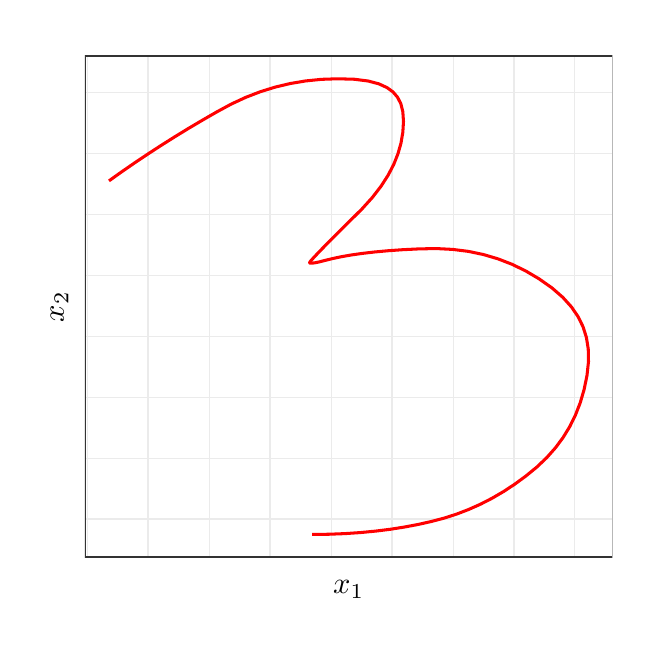
\begin{tikzpicture}[x=1pt,y=1pt]
\definecolor{fillColor}{RGB}{255,255,255}
\path[use as bounding box,fill=fillColor,fill opacity=0.00] (0,0) rectangle (216.81,216.81);
\begin{scope}
\path[clip] (  0.00,  4.73) rectangle (216.81,212.08);
\definecolor{drawColor}{RGB}{255,255,255}
\definecolor{fillColor}{RGB}{255,255,255}

\path[draw=drawColor,line width= 0.6pt,line join=round,line cap=round,fill=fillColor] (  0.00,  4.73) rectangle (216.81,212.08);
\end{scope}
\begin{scope}
\path[clip] ( 20.71, 25.45) rectangle (211.31,206.58);
\definecolor{fillColor}{RGB}{255,255,255}

\path[fill=fillColor] ( 20.71, 25.45) rectangle (211.31,206.58);
\definecolor{drawColor}{gray}{0.92}

\path[draw=drawColor,line width= 0.3pt,line join=round] ( 20.71, 61.20) --
	(211.31, 61.20);

\path[draw=drawColor,line width= 0.3pt,line join=round] ( 20.71,105.24) --
	(211.31,105.24);

\path[draw=drawColor,line width= 0.3pt,line join=round] ( 20.71,149.29) --
	(211.31,149.29);

\path[draw=drawColor,line width= 0.3pt,line join=round] ( 20.71,193.33) --
	(211.31,193.33);

\path[draw=drawColor,line width= 0.3pt,line join=round] ( 21.53, 25.45) --
	( 21.53,206.58);

\path[draw=drawColor,line width= 0.3pt,line join=round] ( 65.57, 25.45) --
	( 65.57,206.58);

\path[draw=drawColor,line width= 0.3pt,line join=round] (109.61, 25.45) --
	(109.61,206.58);

\path[draw=drawColor,line width= 0.3pt,line join=round] (153.66, 25.45) --
	(153.66,206.58);

\path[draw=drawColor,line width= 0.3pt,line join=round] (197.70, 25.45) --
	(197.70,206.58);

\path[draw=drawColor,line width= 0.6pt,line join=round] ( 20.71, 39.18) --
	(211.31, 39.18);

\path[draw=drawColor,line width= 0.6pt,line join=round] ( 20.71, 83.22) --
	(211.31, 83.22);

\path[draw=drawColor,line width= 0.6pt,line join=round] ( 20.71,127.26) --
	(211.31,127.26);

\path[draw=drawColor,line width= 0.6pt,line join=round] ( 20.71,171.31) --
	(211.31,171.31);

\path[draw=drawColor,line width= 0.6pt,line join=round] ( 43.55, 25.45) --
	( 43.55,206.58);

\path[draw=drawColor,line width= 0.6pt,line join=round] ( 87.59, 25.45) --
	( 87.59,206.58);

\path[draw=drawColor,line width= 0.6pt,line join=round] (131.64, 25.45) --
	(131.64,206.58);

\path[draw=drawColor,line width= 0.6pt,line join=round] (175.68, 25.45) --
	(175.68,206.58);
\definecolor{drawColor}{RGB}{255,0,0}

\path[draw=drawColor,line width= 1.1pt,line join=round] (102.76, 33.68) --
	(108.85, 33.76) --
	(114.73, 33.99) --
	(120.40, 34.38) --
	(125.87, 34.91) --
	(131.15, 35.57) --
	(136.24, 36.38) --
	(141.16, 37.31) --
	(145.91, 38.38) --
	(150.51, 39.59) --
	(154.98, 41.03) --
	(159.35, 42.71) --
	(163.63, 44.62) --
	(167.82, 46.77) --
	(171.95, 49.18) --
	(176.01, 51.85) --
	(180.03, 54.80) --
	(183.98, 58.03) --
	(187.56, 61.44) --
	(190.72, 65.00) --
	(193.48, 68.73) --
	(195.89, 72.67) --
	(197.94, 76.85) --
	(199.67, 81.29) --
	(201.06, 86.04) --
	(202.11, 91.14) --
	(202.65, 96.16) --
	(202.56,100.70) --
	(201.90,104.85) --
	(200.69,108.71) --
	(198.90,112.37) --
	(196.49,115.90) --
	(193.37,119.36) --
	(189.43,122.79) --
	(184.74,126.08) --
	(179.93,128.92) --
	(175.01,131.31) --
	(169.95,133.27) --
	(164.73,134.82) --
	(159.31,135.96) --
	(153.64,136.68) --
	(147.68,136.99) --
	(141.45,136.87) --
	(135.57,136.58) --
	(130.20,136.20) --
	(125.32,135.75) --
	(120.91,135.24) --
	(116.94,134.67) --
	(113.37,134.05) --
	(110.20,133.38) --
	(107.39,132.69) --
	(105.15,132.12) --
	(103.64,131.82) --
	(102.69,131.70) --
	(102.18,131.70) --
	(101.96,131.76) --
	(101.89,131.85) --
	(101.91,131.99) --
	(102.09,132.29) --
	(102.53,132.82) --
	(103.25,133.61) --
	(104.29,134.72) --
	(105.71,136.21) --
	(107.59,138.14) --
	(109.97,140.55) --
	(112.93,143.51) --
	(116.52,147.07) --
	(120.73,151.23) --
	(124.54,155.44) --
	(127.69,159.52) --
	(130.25,163.50) --
	(132.28,167.40) --
	(133.81,171.26) --
	(134.90,175.11) --
	(135.56,178.99) --
	(135.80,182.94) --
	(135.55,186.52) --
	(134.82,189.37) --
	(133.64,191.68) --
	(132.01,193.58) --
	(129.81,195.18) --
	(126.89,196.51) --
	(123.04,197.53) --
	(118.04,198.17) --
	(112.04,198.34) --
	(106.15,198.14) --
	(100.43,197.56) --
	( 94.86,196.62) --
	( 89.40,195.32) --
	( 84.04,193.65) --
	( 78.75,191.61) --
	( 73.51,189.17) --
	( 68.30,186.35) --
	( 63.16,183.39) --
	( 58.10,180.40) --
	( 53.12,177.35) --
	( 48.22,174.26) --
	( 43.40,171.13) --
	( 38.65,167.95) --
	( 33.98,164.73) --
	( 29.38,161.45);
\definecolor{drawColor}{gray}{0.20}

\path[draw=drawColor,line width= 0.6pt,line join=round,line cap=round] ( 20.71, 25.45) rectangle (211.31,206.58);
\end{scope}
\begin{scope}
\path[clip] (  0.00,  0.00) rectangle (216.81,216.81);
\definecolor{drawColor}{RGB}{0,0,0}

\node[text=drawColor,anchor=base,inner sep=0pt, outer sep=0pt, scale=  1.10] at (116.01, 12.37) {$x_1$};
\end{scope}
\begin{scope}
\path[clip] (  0.00,  0.00) rectangle (216.81,216.81);
\definecolor{drawColor}{RGB}{0,0,0}

\node[text=drawColor,rotate= 90.00,anchor=base,inner sep=0pt, outer sep=0pt, scale=  1.10] at ( 13.08,116.01) {$x_2$};
\end{scope}
\end{tikzpicture}
